\documentclass[17pt]{extarticle} % another possible option: 20 pt
\usepackage{ifpdf}
\ifpdf
\usepackage{cmap}
\fi
\usepackage[english]{babel}
\usepackage{palatino}
\usepackage[x11names,svgnames]{xcolor}
\usepackage{amsmath,amssymb,amsfonts}
\usepackage{tikz}
\usepackage{amsthm}
\usepackage{enumitem}
%\usepackage{pgf}
%\usepackage{multicol}
\usepackage{xspace}
\usepackage{graphicx}
%\usepackage{multicol}
%\usepackage[section]{algorithm} % [section] is use to define the numbering mode
%\usepackage{algorithmic} 
\usepackage[a1paper,left=2.5cm,right=.5cm,top=2.5cm,bottom=.5cm,foot=0cm]{geometry}
\usepackage{poster}
\usepackage{booktabs}
\usepackage{multirow,multicol}
\usepackage{simplewick}
\DeclareGraphicsExtensions{.png}
\usetikzlibrary{positioning,fadings,fit}

%\usepackage{pgfplots}

%\theoremstyle{definition}
%\newtheorem{definition}{Definition}[section]
%\newtheorem{proposition}{Proposition}[section]
%\newtheorem{corollary}{Corollary}[section]
%\newtheorem{theorem}{Theorem}[section]


\def\myarc#1#2#3#4{
  \draw[color=#1,line width=2pt,->] (360*#2/18:#4mm) arc (360*#2/18:360*#3/18:#4mm);
}%#1 -- color, #2 -- from, #3 -- to, #4 -- radius (mm)

\def\ra{red}
\def\rb{green!50!black}
\def\rc{cyan}
\def\rd{magenta}
\def\re{blue}
\def\rf{orange}

\newcommand{\myignore}[1]{}

\begin{document}
\pagestyle{empty}

%%% RAMKA
%\noindent\hspace{-2cm}
%\begin{tikzpicture}[rounded corners=2cm,x=1cm,y=1cm]
%  \draw (0,-1) [color=SteelBlue3,line width=2mm] rectangle (55.5,79);
%\end{tikzpicture}
%\vspace{-78.5cm}

%%% TITLE
%\begin{center}
  %{\color{OrangeRed} \fontsize{48pt}{1em} {\bf Earmark graph approach to {\it de novo} genome assembly}}
  %\vspace{1.5cm}
    
  %\fontsize{32pt}{2.5em}\selectfont
  %\color{DodgerBlue3}
  %{\bf Mikhail Dvorkin, Alexander S. Kulikov, Max Alekseyev}
  %{affiliations}
  %{\tt emails}
%\end{center}%
%\vspace{1cm}

%\fontsize{32pt}{2.5em}\selectfont

\begin{center}
\begin{tikzpicture}

%%%%%%%%%%%%%%%GRID
%\draw[step=1cm,help lines] (0,0) grid (54,78);
%\foreach \x in {0,...,54} { \node at (\x,-1) {$\x$}; \node at (\x,79) {$\x$}; }
%\foreach \x in {0,...,78} { \node at (-1,\x) {$\x$}; \node at (55,\x) {$\x$}; }

%%%%%%%%%%%%%%%TITLE
\begin{scope}
\draw (0,78) [color=SteelBlue3,line width=2mm,rounded corners=.5cm,fill=blue!10!white] rectangle (54,68);
\node at (27,76) {\color{OrangeRed} \fontsize{45pt}{1em} \bf Expandable de Novo Genome Assembler for Short-Read Sequence Data};
\node[rectangle,text width=16cm,text centered,anchor=north west] at (0,74) {
  {\bf \color{DodgerBlue3} \fontsize{32pt}{1em}\selectfont Nikolay~Vyahhi}
};
\node[rectangle,text width=16cm,text centered,anchor=north west] at (9,74) {
  {\bf \color{DodgerBlue3} \fontsize{32pt}{1em}\selectfont Sergey~Nurk}
};
\node[rectangle,text width=16cm,text centered,anchor=north west] at (18,74) {
  {\bf \color{DodgerBlue3} \fontsize{32pt}{1em}\selectfont Anton~Bankevich}
};
\node[rectangle,text width=16cm,text centered,anchor=north west] at (28,74) {
  {\bf \color{DodgerBlue3} \fontsize{32pt}{1em}\selectfont Max~Alekseyev}
};
\node[rectangle,text width=16cm,text centered,anchor=north west] at (37,74) {
  {\bf \color{DodgerBlue3} \fontsize{32pt}{1em}\selectfont Pavel~Pevzner}
};
\node[rectangle,text width=52cm,text centered,anchor=north west] at (1,72.5) {
  \fontsize{26pt}{1em}\selectfont
  \vspace{7mm}
  Algorithmic Biology Lab, Academic University of the Russian Academy of Sciences, St.~Petersburg, Russia\\
  \vspace{5mm}
  {\tt http://bioinf.spbau.ru/en/assembler}
%  \\[+5mm]
% We've got to include this:
%\small{The presentation of this work was made possible by a Travel Fellowship awarded by ISCB
%with grant funds obtained from the Department of Energy Office of 
%Science,\\
%the National Science Foundation Bio-Directorate,
%and the NIH National Institute of General Medical Sciences.}
};

\end{scope}

%%%%%%%%%%%%%%%PROBLEM STATEMENT AND ABSTRACT
\begin{scope}
\draw ( 0,65) [color=SteelBlue3,line width=2mm,rounded corners=.5cm] rectangle (26,57);
\draw (28,65) [color=SteelBlue3,line width=2mm,rounded corners=.5cm] rectangle (54,58);
\node[draw=SteelBlue3,line width=2mm,rounded corners=.5cm,anchor=south west,fill=blue!10!white,inner sep=3mm] at (28,65) {\fontsize{32pt}{1em} 
\bf In the Poster\phantom{y}};
\node[draw=SteelBlue3,line width=2mm,rounded corners=.5cm,anchor=south west,fill=blue!10!white,inner sep=3mm] at (0,65) {\fontsize{32pt}{1em} 
\bf Abstract\phantom{y}};
\node[rectangle,anchor=west,text width=25cm,inner sep=5mm] at (0,61) {
  De novo genome sequence assembly is the essential step to reveal genomic sequences of different species world-wide. Currently there exists various genome assemblers for short-read NGS data, such as Velvet, SOAPdenovo, ALLPATH, ABySS and others. \newline \newline
 We present new open-source de Bruijn graph-based assembler currently in development on C++, which uses novel algorithmic ideas such as context-free graph approach and also have agile and expandable software architecture. It requires affordable amount of memory and computations while giving high quality results. It provides solid basis for single-cell and mammalian assemblers in the near future.
%  \vspace{5mm}
%  \begin{center}
%   \includegraphics[width=100mm]{logo_blue_white.jpg}
% \end{center}
};
\node[rectangle,anchor=west,text width=25cm,inner sep=5mm] at (28,61.5) {
\begin{enumerate}
\item De Bruijn graph construction, index and callbacks.
\item Error correction and corruption based on topology of the de Bruijn graph (e.g. tip clipping, bulge removal).
\item Efficient data structures for storing and handling of the additional information in the de Bruijn graph (e.g. coverage or distances between pairs of edges).
\end{enumerate}
 };
\end{scope}


%%%%%%%%%%%%%%%CONSTRUCTION
\begin{scope}
  \draw (0,54) [color=SteelBlue3,line width=2mm,rounded corners=.5cm] rectangle (26,47);
  \node[draw=SteelBlue3,line width=2mm,rounded corners=.5cm,anchor=south west,fill=blue!10!white,inner sep=3mm] at (0,54) {\fontsize{32pt}{1em} \bf 
    Graph Construction\phantom{y}};
 \node[rectangle,anchor=west,text width=24cm,inner sep=5mm] at (0,50.5) {
\begin{itemize}
\item Vetexes: $K$-mers. Edges: $(K+1)$-mers.
\item All simple pathes (i.e. without branchings) are condensed.
\item Hash-index $(K+1)$-mer $\rightarrow (edge, offset)$.
\item 2 bits per nucleotide in sequences.
\item Every edge/vertex knows it's reverse-complementary edge/vertex.
\end{itemize}
 };    
\end{scope}

%%%%%%%%%%%%%%%OPERATIONS
\begin{scope}
  \draw (28,55) [color=SteelBlue3,line width=2mm,rounded corners=.5cm] rectangle (54,45);
  \node[draw=SteelBlue3,line width=2mm,rounded corners=.5cm,anchor=south west,fill=blue!10!white,inner sep=3mm] at (28,55) {\fontsize{32pt}{1em} \bf 
    Graph Operations\phantom{y}};
 \node[rectangle,anchor=west,text width=24cm,inner sep=5mm] at (28,50) {
\begin{itemize}
\item \textbf{\color{OrangeRed}Addition/deletion of edge/vertex}.
\item \textbf{\color{OrangeRed}Concatenation of a path}.
\item \textbf{\color{OrangeRed}Split of an edge} in a given position.
\item \textbf{\color{OrangeRed}Projection of one edge} (with all additional info) to another edge.
\end{itemize}
Callback technique: each time a modifying operation is performed corresponding event is triggered and all objects that listen to graph events are notified about what exactly happened to the graph. It allows to implement any additional information as an external structure and hide its logic from the graph and from processing algorithms.

 };    
\end{scope}

%%%%%%%%%%%%%%%ERRORS
\begin{scope}
  \draw (0,44) [color=SteelBlue3,line width=2mm,rounded corners=.5cm] rectangle (35,35);
  \node[draw=SteelBlue3,line width=2mm,rounded corners=.5cm,anchor=south west,fill=blue!10!white,inner sep=3mm] at (0,44) {\fontsize{32pt}{1em} \bf 
    Error Handling\phantom{y}};
 \node[rectangle,anchor=west,text width=34cm,inner sep=5mm] at (0,39.5) {
\begin{itemize}
\item \textbf{\color{OrangeRed}Tip Clipping}. \\
We iterate through all edges of the de Bruijn graph in order of increasing length. \\
If current edge topologically looks like tip and has alternative path with good enough $coverage$ this edge will be removed.
\item \textbf{\color{OrangeRed}Simple Bulge Removal}. \\
Simple bulge is a rather short edge $e$ with an alternative path $P$ between its start and end of length $\approx length(e)$ \\
Our current approach is iterative removal of simple bulges. This strategy allows to delete pretty complex bulge structures and appeared to work pretty well if we alternate it with low coverage edge removal.
\item \textbf{\color{OrangeRed}Removal of Low-Coverage Edges} with small length (as erroneous).
\end{itemize}
 };
\end{scope}

%%%%%%%%%%%%%%%INFO
\begin{scope}
  \draw (0,32) [color=SteelBlue3,line width=2mm,rounded corners=.5cm] rectangle (35,24);
  \node[draw=SteelBlue3,line width=2mm,rounded corners=.5cm,anchor=south west,fill=blue!10!white,inner sep=3mm] at (0,32) {\fontsize{32pt}{1em} \bf 
    Additional Info\phantom{y}};
 \node[rectangle,anchor=west,text width=34cm,inner sep=5mm] at (0,28) {
\begin{itemize}
\item \textbf{\color{OrangeRed}Coverage}. \\
For edge it's the number of $(K+1)$-mers from this edge which was in initial genomic reads. \\
Coverage is additive, means sum of coverages of two edges is the coverage of the concatenation of this two edges.
\item \textbf{\color{OrangeRed}Distances} between edges (usually takes from mate-reads or long reads).
$$(edge, edge, distance) \rightarrow level~of~certainty~(weight)$$
Insert length has large dispersion value thus clustering of some sort is required. There are two types of clustering each of which are implemented: online clustering and offline clustering.
\end{itemize}
 };
\end{scope}

%%%%%%%%%%%%%%%EXAMPLE
%\begin{scope}[yshift=-7cm]
%  \draw (0,60) [color=SteelBlue3,line width=2mm,rounded corners=.5cm] rectangle (54,32);
%  \node[draw=SteelBlue3,line width=2mm,rounded corners=.5cm,anchor=south west,fill=blue!10!white,inner sep=3mm] at (0,62) {\fontsize{32pt}{1em} \bf 
% Goals};
%
%  \node[rectangle,draw=SteelBlue3,line width=3pt,fill=white,anchor=north west,text width=8cm,rounded corners=.5cm,inner sep=3mm] at (0.5,61.5) {\fontsize{26pt}{1em} \bf In this example:\\ $r=8$\\ $k=4$};
%  

%
%  %%% READS
%  \node[rectangle,line width=2pt,text width=5cm,text centered,anchor=west] (reads) at (1,48.5) {
%    {\bf set ${\cal R}$ of reads of length $r$}\\
%    {\color{\ra}  $R_1$: $\overrightarrow{\tt CATGTAGT}$}\\
%    {\color{\rb}  $R_2$: $\overrightarrow{\tt GTAACATG}$}\\
%    {\color{\rc}  $R_3$: $\overrightarrow{\tt AGTGTACA}$}\\
%    {\color{\rd}  $R_4$: $\overrightarrow{\tt TGTAGTGT}$}\\
%    {\color{\re}  $R_5$: $\overrightarrow{\tt CATGTAAC}$}\\
%    {\color{\rf}  $R_6$: $\overrightarrow{\tt TAACATGT}$}\\
%  };
%
%  \begin{scope}[xshift=48.5cm,yshift=48.5cm,scale=1.2,transform shape]
%    \node (genometop)  at (0,3.5) {};
%    \node (genomedown) at (0,-3.5) {};
%    \node (genomeleft) at (-3.5,0) {};
%
%    \foreach \i/\a in {0/C,1/A,2/T,3/G,4/T,5/A,6/A,7/C,8/A,9/T,10/G,11/T,12/A,13/G,14/T,15/G,16/T,17/A} {
%      \node[fill=white] at (360*\i/18:2cm) {${\tt \a}$};
%      %\node at (360*\i/18:1.5cm) {{\small \i}};
%    }
%    \node at (0,0) {genome $S$};
%    %\draw[color=red,->] (360*5/18:2.2cm) arc (360*5/18:360*11/18:2.2cm);
%    %\myarc{black}{1}{18}{16}
%    \myarc{\ra}{7}{14}{24}  %R1
%    \myarc{\rb}{3}{10}{26}  %R2
%    \myarc{\rc}{-6}{1}{28}  %R3
%    \myarc{\rd}{9}{16}{30}  %R4
%    \myarc{\re}{0}{7}{32}   %R5
%    \myarc{\rf}{3}{10}{34}  %R6
%  \end{scope}
%
%  %\draw [->,line width=2pt] (reads) to[out=90,in=180] node[sloped,fill=white] {de Bruijn graph} (23,53);
%  %\draw [->,line width=2pt] (reads) to[out=-90,in=180] node[sloped,fill=white] {earmark graph} (23,44);
%
%
%  \begin{scope}[scale=1.3,transform shape,line width=2pt]
%    \begin{scope}[xshift=18cm,yshift=40cm]
%      \foreach \x/\y/\t in {0.5/4.5/CATG, 2.5/3.5/ATGT, 4/3/TGTA, 5.5/3/GTAG, 5.5/1.5/GTAA,
%        7/4/GTAC, 7/3/TAGT, 7/0.5/TAAC, 9/3/AGTG, 9/0.5/AACA, 10.5/4/TACA, 10.5/2.5/GTGT, 12/4/ACAT}
%      \node[draw,rectangle,scale=0.7] (\t) at (\x,\y) {${\tt \t}$};
%
%      \foreach \s/\t in {TAGT/AGTG, AGTG/GTGT, TGTA/GTAA, GTAC/TACA, TACA/ACAT}
%        \draw [->] (\s) to (\t);
%      \draw [->] (GTGT) to[bend left=20] (TGTA);
%      \draw [->] (TGTA) to[bend left=20] (GTAC);
%      
%      \foreach \s/\t in {CATG/ATGT,ATGT/TGTA,TGTA/GTAG,GTAG/TAGT}
%        \draw [->,color=\ra] (\s) to (\t);
%      \foreach \s/\t in {GTAA/TAAC, TAAC/AACA}
%        \draw [->,color=\rb] (\s) to (\t);
%      \draw [->,color=\rb] (AACA) to[bend right=45] (ACAT);
%      \draw [->,color=\rb] (ACAT) to[bend right=20] (CATG);
%
%      \node[rectangle,fit=(CATG) (ACAT) (AACA)] (debruijngraph) {};
%    \end{scope}
%
%    \begin{scope}[xshift=18cm,yshift=29cm]
%      \foreach \x/\y/\t in {0.5/4.5/CATG, 5.5/1.5/GTAA,
%        7/3/TAGT, 9/3/AGTG, 10.5/4/TACA, 12/4/ACAT}
%      \node[draw,rectangle,scale=0.7] (\t) at (\x,\y) {${\tt \t}$};
%
%      \foreach \x/\y/\t in {2.5/3.5/ATGT, 4/3/TGTA, 5.5/3/GTAG, 
%        7/4/GTAC, 7/0.5/TAAC, 9/0.5/AACA, 10.5/2.5/GTGT}
%      \node[draw=black!30,rectangle,scale=0.7] (\t) at (\x,\y) {${\tt \textcolor{black!30} \t}$};
%
%      \foreach \s/\t in {TAGT/AGTG, AGTG/TACA}
%        \draw [->] (\s) to (\t);
%      \draw [->] (CATG) to[bend right=20] (GTAA);
%      \draw [->,color=\rb] (GTAA) to[bend right=40,in=-90] (ACAT);
%      \draw [->,color=\rb] (ACAT) to[bend right=20] (CATG);
%      \draw [->,color=\ra] (CATG) to[bend left=5] (TAGT);
%      \draw [->] (TACA) to[bend right=15] (CATG);
%
%      \node[rectangle,fit=(CATG) (ACAT) (AACA)] (earmarkgraph) {};
%    \end{scope}
%  \end{scope}
%
%  %\node[anchor=south west,scale=0.5] (debruijngraph) at (30,51) {\includegraphics{de.pdf}};
%  %\node[anchor=south west,scale=0.5] (earmarkgraph)  at (30,37) {\includegraphics{en.pdf}};
%
%  \node[rectangle,line width=2pt,text width=3cm,text centered,anchor=west] (earmarks) at (9,38) {
%    {\bf earmarks}\\
%    ${\tt CATG}$ ${\tt TACA}$\\
%    ${\tt GTAA}$ ${\tt ACAT}$\\
%    ${\tt AGTG}$ ${\tt TAGT}$
%  };
%
%  \node[rectangle,line width=2pt,text width=5cm,text centered,anchor=west] (earmarkedreads) at (15,38) {
%    {\color{\ra} $R_1: \contraction{}{\tt C}{\tt AT}{\tt G}%
%    \contraction{\tt CATG}{\tt T}{\tt AG}{\tt T}%
%    {\tt CATGTAGT}$ }
%
%    {\color{\rb} $R_2: \contraction{}{\tt G}{\tt TA}{\tt A}%
%    \contraction{\tt GTA}{\tt A}{\tt CA}{\tt T}%
%    \bcontraction{\tt GTAA}{\tt C}{\tt AT}{\tt G}%
%    {\tt GTAACATG}$ }
%
%    {\dots}
%  };
%
%  \begin{scope}[draw=SteelBlue3,line width=3pt,fill=white]
%    \draw [->] (reads) to[out=90,in=180] node[fill=white,rectangle,text width=5cm] 
%      {\color{DodgerBlue3} 1. represent each read as a path on its $r-k+1$ consecutive \mbox{$k$-mers}} (debruijngraph);
%
%    \draw [->] (debruijngraph) to[out=15,in=90] node[fill=white,sloped,rectangle,text width=7cm] 
%      {\color{DodgerBlue3} 2. simplify the graph (compress simple paths, clip tips, remove erroneous connections and bulges) and find a cycle containing all the edges} (genometop);
%
%    \draw [->] (reads) to[out=-90,in=180] node[fill=white,sloped,rectangle,text width=5cm] 
%      {\color{DodgerBlue3} 1. construct a set ${\cal E} \subseteq \{{\tt A,C,G,T}\}^k$ of earmarked \mbox{$k$-mers} such that each read contains at least
%      two earmarked $k$-mers} (earmarks);
%
%    \draw [->] (earmarks) to[out=-90,in=-90] node[fill=white,rectangle,text width=6cm] 
%      {\color{DodgerBlue3} 2. find the earmarks in the reads} (earmarkedreads);
%
%    \draw [->] (earmarkedreads) to[out=-45,in=-135] node[fill=white,rectangle,text width=5cm] 
%      {\color{DodgerBlue3} 3. represent each read as a path on its consecutive earmarks} (earmarkgraph);
%
%    \draw [->] (earmarkgraph) to[out=-30,in=-90] node[fill=white,sloped,rectangle,text width=7cm] 
%      {\color{DodgerBlue3} 4. simplify the graph (compress simple paths, clip tips, remove erroneous connections and bulges) and find a cycle containing all the edges} (genomedown);
%  \end{scope}
%
%  \node at (30,60) {\fontsize{26pt}{1em} \color{OrangeRed} \bf (standard) de Bruijn graph approach};
%  \node at (30,33) {\fontsize{26pt}{1em} \color{OrangeRed} \bf (new) earmark graph approach};
%  %\draw[color=OrangeRed,dashed,line width=5pt,->] (7,48) node[above] {genome assembly problem} -- (46,48);
%  \path (reads) edge[color=OrangeRed,dashed,line width=5pt,->] node[above] {\fontsize{26pt}{1em} \color{OrangeRed} \bf \emph{de novo} genome assembly problem} (genomeleft);
%\end{scope}

%%%%%%%%%%%%%%%ADVANTAGES
%\begin{scope}
%  \draw (0,22) [color=SteelBlue3,line width=2mm,rounded corners=.5cm] rectangle (30,0);
%  \node[draw=SteelBlue3,line width=2mm,rounded corners=.5cm,anchor=south west,fill=blue!10!white,inner sep=3mm] at (0,22) {\fontsize{32pt}{1em} \bf 
%    Advantages of earmark graph over de Bruijn graph};
%  \node[rectangle,text width=28cm,anchor=west] at (1,11) {
%    \fontsize{24pt}{1em}\selectfont
%    %TO BE REWRITTEN
%    \begin{description}
%    \item[\color{OrangeRed} \bf Smaller size.]
%    The earmark graph requires less time and memory for construction.
%    Note also that one can control the size of the earmark graph 
%    by varying the size of the set of earmarks. Also, it is easy to see 
%    that in an extreme case when ${\cal E}$ is just the set of all the 
%    $k$-mers of the input reads, the earmark graph coincides with the de 
%    Bruijn graph.
%    \item[\color{OrangeRed} \bf Simpler structure.]
%    In the example above, the de Bruijn graph contains two vertices $v$ with 
%    $\textrm{indegree}(v)\times\textrm{outdegree}(v) \ge 2$, while the 
%    earmark graph contains only one such vertex. 
%    This corresponds to a simpler representation of repeats 
%    in the genome and simplifies the problem of finding a cycle in the 
%    graph.
%    %At the same time, the 
%    %genome can be spelled through both graphs.
%    %To give an example, consider two reads ${\tt TTGCAC}$ and ${\tt 
%    %ATGCAT}$ sharing a $4$-mer ${\tt TGCA}$. They are represented as two paths, shown 
%    %in Fig.~\ref{fig:repa}, in the de Bruijn graph built on $3$-mers
%    %(this is a part of the de Bruijn graph from Fig.~\ref{fig:debruijn}).
%    %This is a typical repeat. The edge ${\tt TGC}\rightarrow{\tt GCA}$ has two
%    %incoming edges and two outgoing edges. While spelling a genome
%    %through this part of the graph it is not clear which incoming edge 
%    %corresponds to which outgoing edge. However in the earmarked graph
%    %this repeat may be already resolved if the $3$-mers {\tt TGC} and {\tt GCA}
%    %are not earmarked, see Fig.~\ref{fig:repb}.
%    \item[\color{OrangeRed} \bf Using trusted $k$-mers.] 
%    By restricting earmarks to $k$-mers present in many reads (``trusted'' $k$-mers)
%    one can reduce the number of erroneous edges resulting from 
%    sequencing errors in the reads.
%    \end{description}
%  };
%\end{scope}

%%%%%%%%%%%%%%%PRACTICAL RESULTS
%\begin{scope}
%  \draw (0,18) [color=SteelBlue3,line width=2mm,rounded corners=.5cm] rectangle (18,0);
%  \node[draw=SteelBlue3,line width=2mm,rounded corners=.5cm,anchor=south west,fill=blue!10!white,inner sep=3mm] at (0,18) {\fontsize{32pt}{1em} \bf 
%    Dataset\phantom{y}};
%  
%\node[rectangle,anchor=west,text width=18cm,inner sep=5mm] at (0,9) {
%
%};
%\end{scope}

%%%%%%%%%%%%%%%EVALUATIONS

 \node[rectangle,anchor=west,text width=16cm,inner sep=5mm] at (17,16.5) {
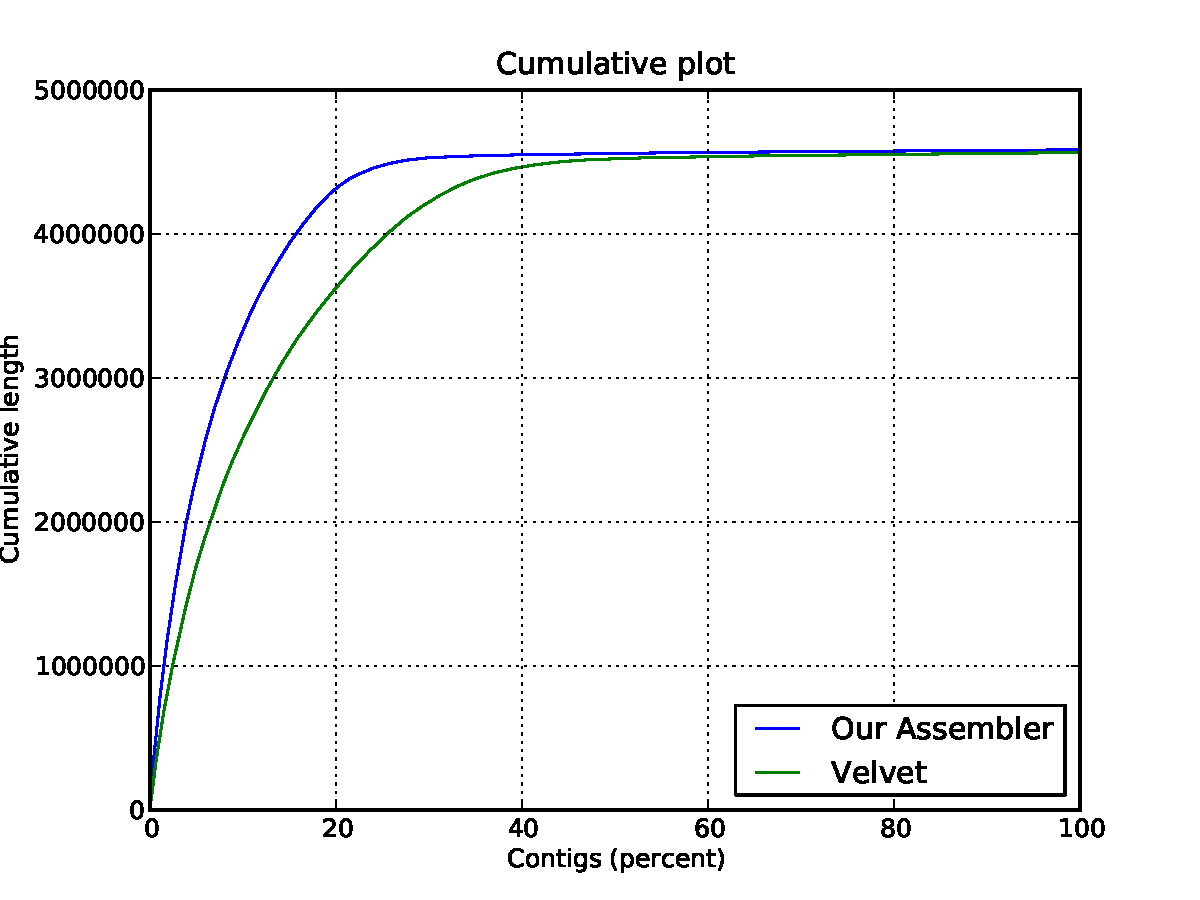
\includegraphics[height=13.75cm]{cumulative_plot.pdf}
 };
 
  \node[rectangle,anchor=west,text width=16cm,inner sep=5mm] at (-1,6.5) {
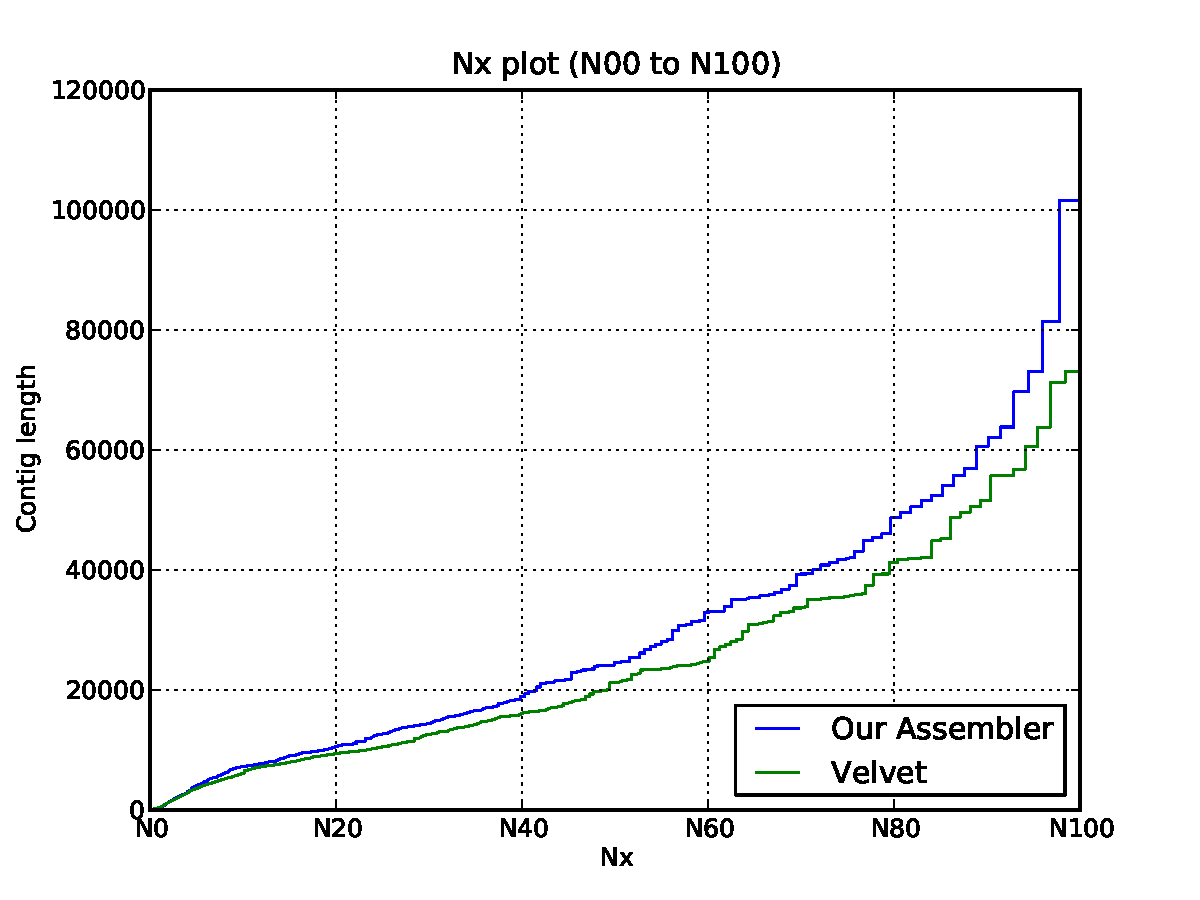
\includegraphics[height=13.75cm]{Nx_plot.pdf}
 };
 
 \node[rectangle,anchor=west,text width=18cm,inner sep=5mm] at (35,26) {
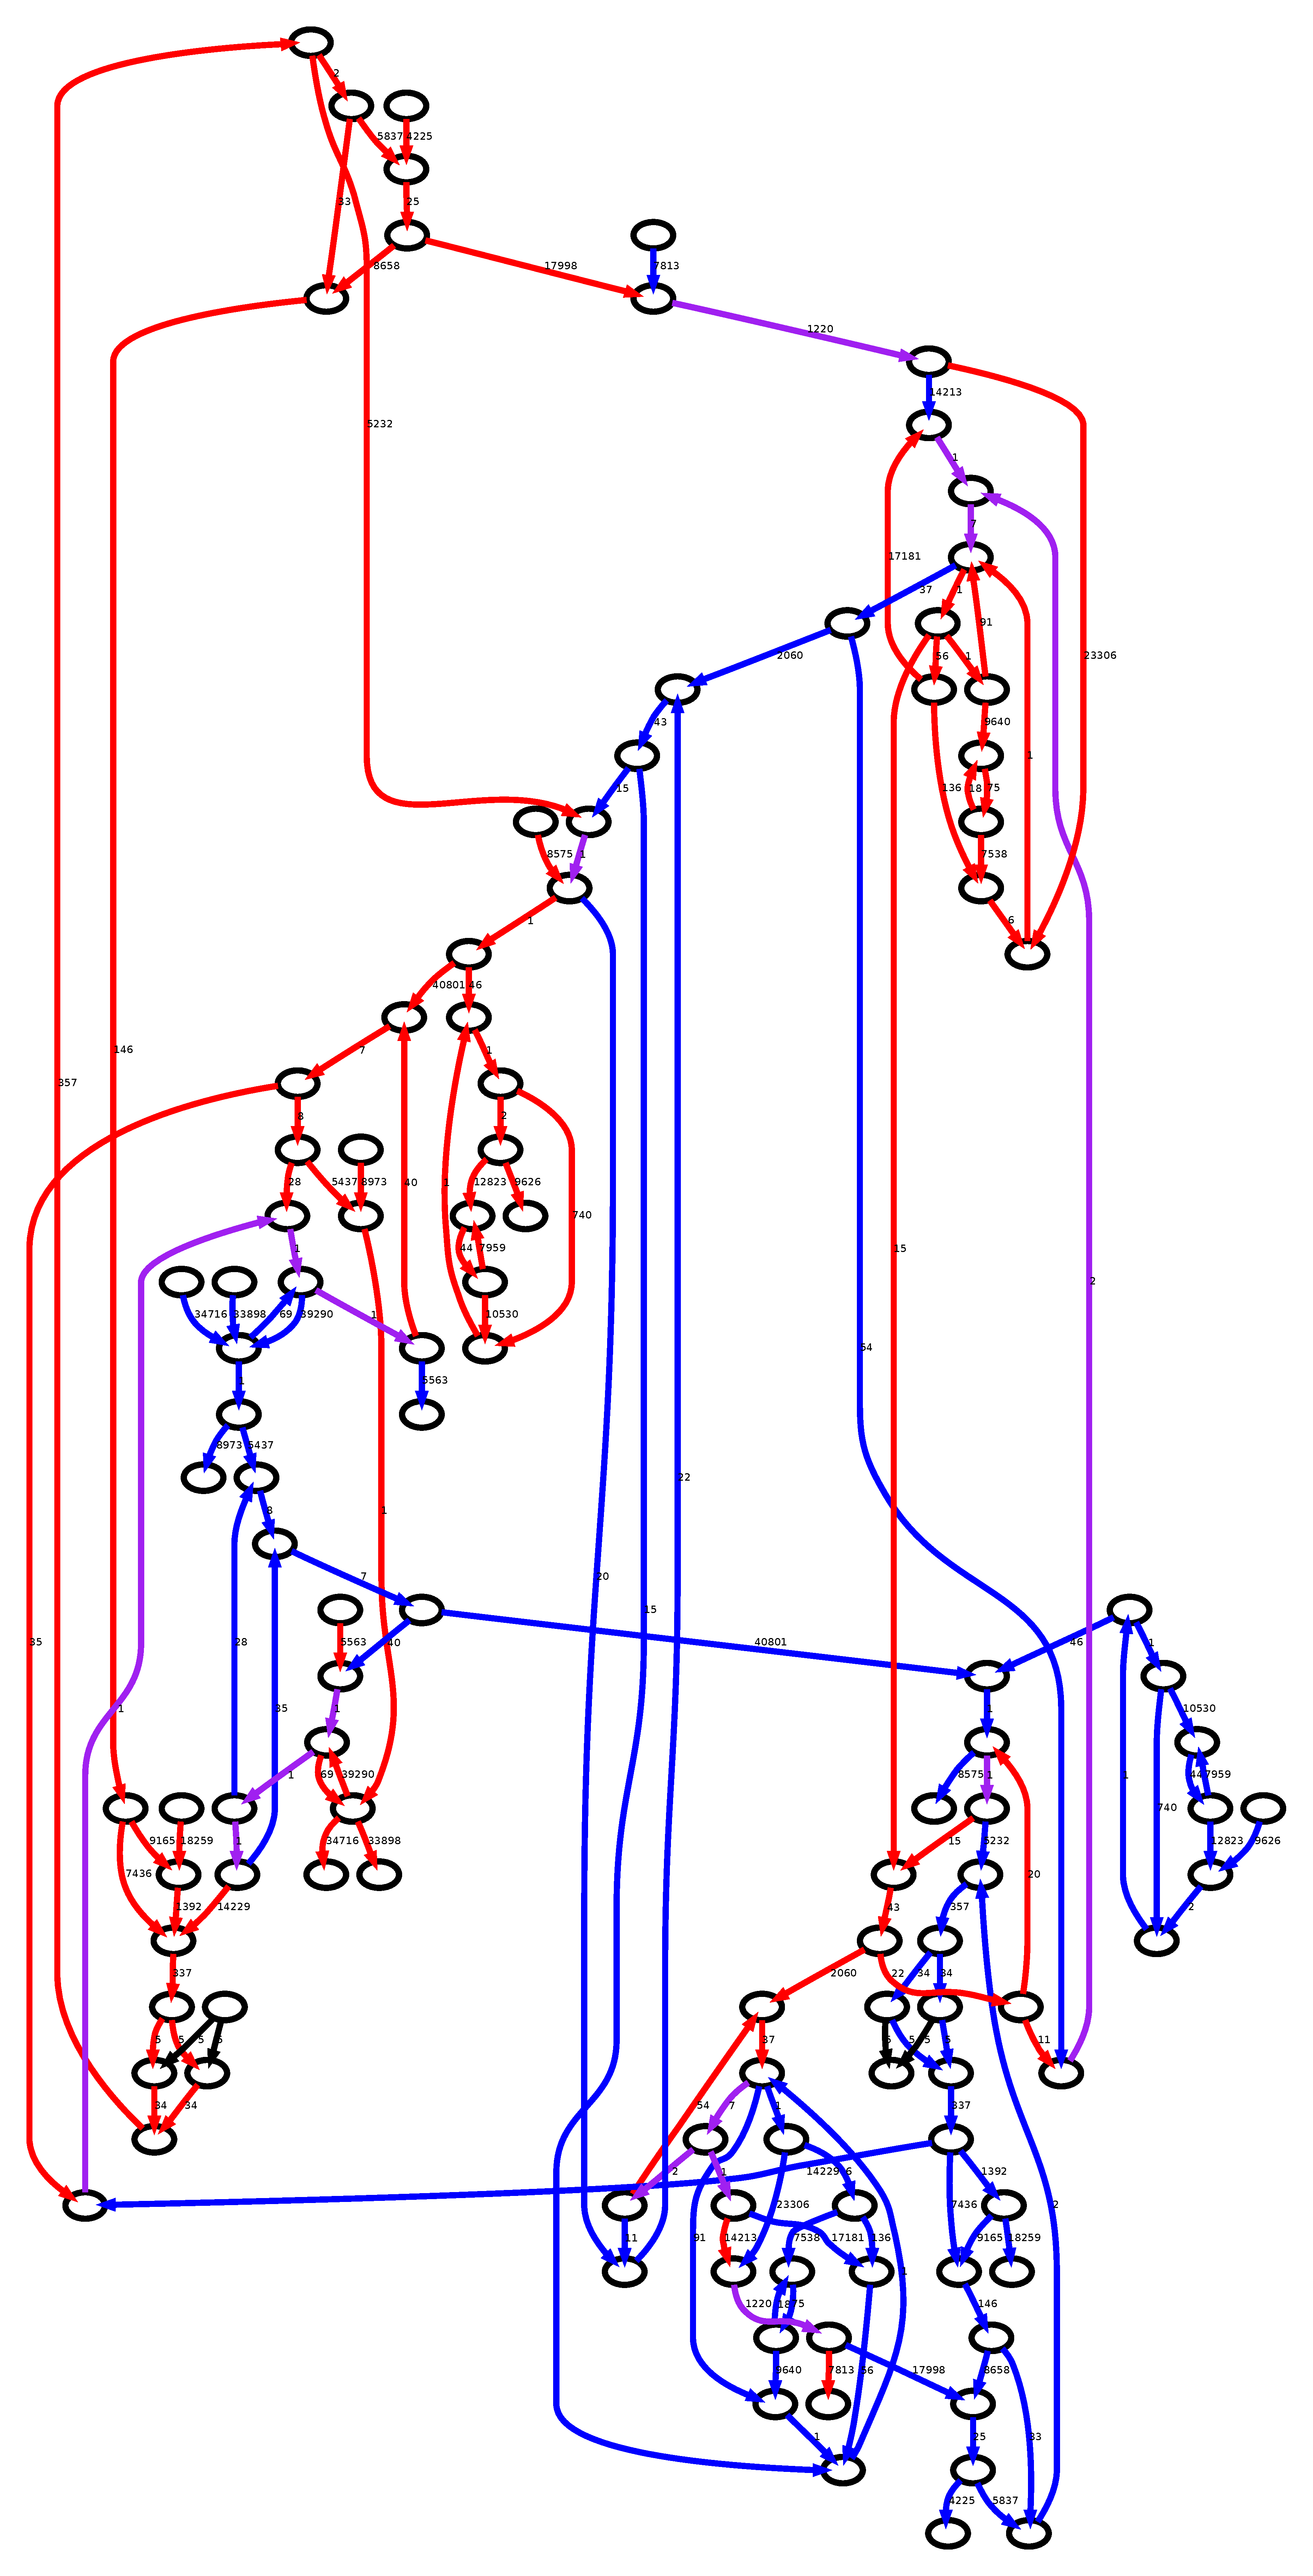
\includegraphics[width=19cm]{graph_simple2.pdf}
 };

%%%%%%%%%%%%%%%DATASET
\begin{scope}
  \draw (0,21) [color=SteelBlue3,line width=2mm,rounded corners=.5cm] rectangle (16,14);
  \node[draw=SteelBlue3,line width=2mm,rounded corners=.5cm,anchor=south west,fill=blue!10!white,inner sep=3mm] at (0,21) {\fontsize{32pt}{1em} \bf 
    Evaluation\phantom{y}};
\node[rectangle,anchor=west,text width=15cm,inner sep=5mm] at (0,17.5) {
\begin{itemize}
\item \textbf{E.Coli} MG1655-K12 bacteria (4.6Mbp genome)
\item 14M Illumina paired-end reads of \\ size = 100bp, gap $\approx$ 20bp (total: \textbf{6 Gb of FASTQ}).
\item Error Correction with Quake (before assembly).
\item $\approx$ \textbf{1 hour} on a laptop, 1 Gb RAM, no HDD.
\end{itemize}
 };
\end{scope}

%%%%%%%%%%%%%%%FUTURE
\begin{scope}
  \draw (17,8) [color=SteelBlue3,line width=2mm,rounded corners=.5cm] rectangle (35,0);
  \node[draw=SteelBlue3,line width=2mm,rounded corners=.5cm,anchor=south west,fill=blue!10!white,inner sep=3mm] at (17,8) {\fontsize{32pt}{1em} \bf 
    Future\phantom{y}};
\node[rectangle,anchor=west,text width=17cm,inner sep=5mm] at (17,4) {
\begin{enumerate}[start=0]
\item \textbf{\color{OrangeRed}Repeats resolving}.
\item \textbf{\color{OrangeRed}Single Cell} (Bacterial) Assembler.
\item \textbf{\color{OrangeRed}Mammalian} Genomes Assembler (see the poster of \textit{Mikhail Dvorkin} and \textit{Alexander Kulikov}: Earmark graph approach to de novo genome assembly).
\item \textbf{\color{OrangeRed}Transcriptome} Assembler, \textbf{\color{OrangeRed}Cancer Genomes} Assembler and other customizations...
\end{enumerate}
 };
\end{scope}


%%%%%%%%%%%%%%%TEAM
\begin{scope}
  \draw (36,6) [color=SteelBlue3,line width=2mm,rounded corners=.5cm] rectangle (54,0);
  \node[draw=SteelBlue3,line width=2mm,rounded corners=.5cm,anchor=south west,fill=blue!10!white,inner sep=3mm] at (36,6) {\fontsize{32pt}{1em} \bf 
    Team\phantom{y}};
\node[rectangle,anchor=west,text width=17cm,inner sep=5mm] at (36,3) {
\color{DodgerBlue3}Dmitrij Antipov, Anton Bankevich, Mikhail Dvorkin, \\ Alexander Kulikov, Sergey Nurk, Alexander Sirotkin, \\ Nikolay Vyahhi, Max Alekseyev, Pavel Pevzner. \newline \newline
Supported by "megagrant"\\(The Ministry of Education and Science, Russia).
};
\end{scope}

\end{tikzpicture}
\end{center}


\end{document}
